\chapter{Future Scope and Conclusion}
\label{chap:conclusion}


%%%%%%%%%%%%%%%%%%%%%%%%%%%%%%%%%%%%%
%%%%%%%%%%%%%%%%%%%%%%%%%%%%%%%%%%%%%
%%%%%%%%%%%%   SECTION   %%%%%%%%%%%%
%%%%%%%%%%%%%%%%%%%%%%%%%%%%%%%%%%%%%
%%%%%%%%%%%%%%%%%%%%%%%%%%%%%%%%%%%%%
\section{Some Implementation Details}
\label{sec:ch5:hurdles}
The whole application is written in \verb|C| and uses \verb|pthread, SQLite, FFTW| external libraries for computation as well as storing the execution measurement results. Some of the important challenges faced during the implementation phase are listed here.

\subsection{Synchronization}
\verb|wait_for_all_threads()| function (Appendix \ref{app:code:wait_for_others}) is providing a synchronization point. Sync point is provided at the beginning of every benchmark (3xCMYACC, 4xRMY, etc) execution to make sure that threads are running simultaneously. A thread reaching this function first locks the mutex variable \verb|mutex| then waits on condition variable \verb|cv_count|. The last(4$^{th}$) thread reaching this function will release the condition variable by broadcasting followed by releasing the mutex \verb|mutex|. Now one thread(4$^{th}$) has passed the synchronization point and remaining three threads are waiting for the \verb|mutex| access, called thread wakeup. Those waiting three threads will be released one after another serially. In the program execution, there may be a scenario where the first thread crossing the sync point-1 will reach sync point-2 \verb|wait_for_all_threads()| and waits for the \verb|mutex| access, before all the three threads are released from sync point-1.

\begin{figure}[h!]
	\centering
	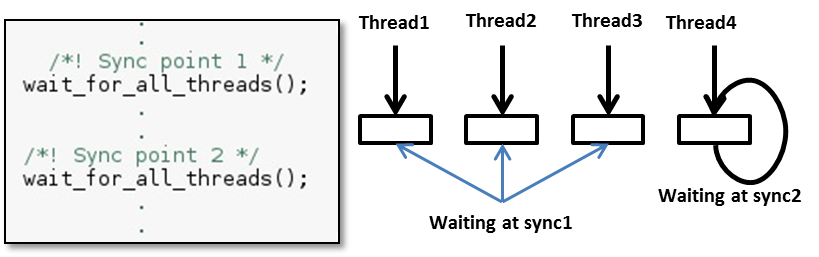
\includegraphics[width=140mm]{figures/wait_for_all_threads}
	\caption{Race Condition in wait\_for\_all\_threads() Function}
	\label{fig:conclusion:thread_wakeup}
\end{figure}

Figure \ref{fig:conclusion:thread_wakeup}, illustrates the first three threads are waiting at sync1, while the 4$^{th}$ thread crossed sync-1 and waiting for \verb|mutex| access corresponds to sync-2. On such occasions, the order of thread wakeup relies on the scheduling policy of the thread \cite{pthreadWait}. This goes haywire in a multithreaded environment where the order of thread execution is non deterministic. This issue occurred at sporadic intervals making it hard to debug. Validating the number of awakened threads solved the problem. It acts as a guard for mutex lock mechanism. 

\subsection{Thread Safety}
The benchmarks should be thread-safe to be executed in parallel threads. FFTW has \verb|fftw_plan| stage to prepare input parameters of \verb|fftw_execute|. According to the FFTW documentation, \verb|fftw_execute| is thread-safe, but not \verb|fftw_plan| \cite{fftThreadSafe}. However, the same plan can be used for multiple threads in parallel. Instead of all threads executing \verb|fftw_plan|, only one thread is allowed to execute \verb|fftw_plan|, then all threads are allowed to do \verb|fftw_execute| in parallel. \vspace*{0.3cm}

\subsection{Performance of the SQLite Library}
SQLite library is used to store execution time measurements of the Radar benchmarks into a database. The Radar algorithm has ten performance critical functions as benchmarks. Every thread will store the execution measurement result at the end of every benchmark processing. The SQLite library performs well in a single threaded application with relatively less number of insertions. The scene is extremely different in a multithreaded environment. Data insertions have to be mutually exclusive as only one database is used through the application. Four threads, running on four cores inserting 40,000 records consumed 15 hours on ARM Cortex A9 platform. Retrieval is also equally slow. On the other hand, \verb|.csv| implementation of the same did it in couple of minutes. Processing \verb|.csv| data is also simple and convenient as it can be interpreted by Microsoft Excel.


%%%%%%%%%%%%%%%%%%%%%%%%%%%%%%%%%%%%%
%%%%%%%%%%%%%%%%%%%%%%%%%%%%%%%%%%%%%
%%%%%%%%%%%%   SECTION   %%%%%%%%%%%%
%%%%%%%%%%%%%%%%%%%%%%%%%%%%%%%%%%%%%
%%%%%%%%%%%%%%%%%%%%%%%%%%%%%%%%%%%%%
\section{Future Scope}
There are lot of scopes for fine tuning the application and extending this research work. Some of them are discussed below.

\subsection{Parallel Executable Modules}
Latency reduction is greatly influenced by the amount of parallelism available in the application. Among the A/A mode benchmarks, Convolution and FFT are the major latency contributors. Scheme-4 executes FFTW library for every channel (Sum, Guard, Azimuth and Elevation) in sequential order, whilst Scheme-5 performs channel computations in parallel. In any case, single instance of FFT library is executed in serial. Breaking the FFT and Convolution benchmarks into parallel executable modules will allow greater improvement of execution time. This enables more than one core performing FFT computation of one channel, resulting in speedup factor of broken parallel modules. \vspace*{0.2cm}

Benchmarks like Complex Multiply Accumulate (CMYACC), Range Multiply (RMY), Magnitude (MAG), Area Average Calculation (AVG) and Comparison (CMPR) have lot amount of parallelism. Loop iterations in the above benchmarks can be split to run in parallel. Effective speedup will be equal to number of parallel executable modules. Although breaking the application for parallel execution increases speedup, it needs more computing entities to carry out the task, new data distribution schemes and so mode mapping. This is a starting point of the optimization and requires further feasibility study.

\subsection{Architectural Features}
The \verb|FFTW| library might not have used special architecture features, since regardless of turning on the \verb|arm| specific compiler switches, it complained 
\begin{compactitem}
	\item[] \verb|not vectorized: not enough data-refs in basic block.|
	\item[] \verb|not vectorized: failed to find SLP opportunities in basic block.|
\end{compactitem}
So it is not optimized for ARM Cortex A9 platform. 128-bit advanced SIMD unit of the ARM Cortex A9 processor can perform four math operations of 32-bit data at the cost of one math operation. Exploiting such feature will reduce the latency of the computation heavy modules in single threaded as well as multi-threaded environment.

\subsection{Cache Performance}
The more the cache hit rate, the less the memory transfer between SDRAM and core. Fetching data from memory is relatively slow and expensive. Corner turning is implemented as generic row-column transpose form. The data access pattern row-column wise, makes frequent cache misses. Corner turning can be implemented by Cache-Oblivious Algorithm as explained in \textsl{Cache Oblivious Matrix Transposition:Simulation and Experiment} \cite{cot}, to improve data locality. This will reduce memory transfer bandwidth as well as execution time.  \vspace*{0.2cm}

In Scheme-5, the burst data size after beamforming is 52KiB. A core having 32KiB private L1 cache can hold up to 61\% of the beamformed data. As an over approximation approach, 0\% cache hit rate is assumed for the analysis. This is not the case in real world. Cache hit rate prediction mechanism shall be employed to have more realistic results. \vspace*{0.2cm}

Effect of various L2-Cache size and Memory size can be performed to determine the optimal size for working set data. Another interesting cache profiling is \textsl{cache data utilization ratio}, it is the ratio of the amount of data fetched from memory to the amount of data used by the CPU before the data is evicted. Such measurements in L1 cache and L2 cache indicate whether changes in the algorithm will yield significant reduction in execution time.

\subsection{A/G Mode}
This thesis has only considered A/A Mode processing of the Radar processor. The techniques shall be extended to adopt A/G Mode processing. A Radar processor should be capable of performing A/A Mode and A/G Mode processing in real time.

%\clearpage
\section{Conclusion}
\label{sec:ch5:conclustion}
This thesis has presented the Airborne Radar processing chain, IMA processor architecture for safety critical systems and existing mode mapping analysis. Inference from the existing analysis is that the latency is far higher than the acceptable values. Data dependency is scrutinized to leverage parallelism in the application. Pseudo algorithm of the Radar processing chain is implemented and the latency is measured on a real hardware. Measurement tools for memory utilization and bandwidth utilization have been made. \vspace*{0.2cm}

Couple of optimization schemes have been implemented for Air to Air Mode processing. Based on the new mode mapping analysis, the optimized scheme(Scheme-4) guarantees 7.5x speedup than the existing analysis with lesser number of resources. The achieved 2x dwell latency is healthy enough for the A/A Mode Radar processor. \vspace*{0.2cm}

This thesis concludes that the simplified A/A mode Radar processing can be done on the IMA processer architecture in real time. It saves space, weight and power requirements. To compare this in day to day life, eight Samsung Galaxy S-III mobiles are sufficient to deliver 2x dwell latency with 87\% CPU utilization!

%Transforming development stage to the production stage will rip out the complex operating system, unnecessary interfaces and unused modules from the hardware platform. This will minimize some overhead in processing. \\